%%%%%%%%%%%%%%%%%%%%%%%%%%%%%%%%%%%%%%%%%
% Beamer Presentation
% LaTeX Template
% Version 1.0 (10/11/12)
%
% This template has been downloaded from:
% http://www.LaTeXTemplates.com
%
% License:
% CC BY-NC-SA 3.0 (http://creativecommons.org/licenses/by-nc-sa/3.0/)
%
%%%%%%%%%%%%%%%%%%%%%%%%%%%%%%%%%%%%%%%%%

%----------------------------------------------------------------------------------------
%	PACKAGES AND THEMES
%----------------------------------------------------------------------------------------

\documentclass{beamer}

\mode<presentation> {

% The Beamer class comes with a number of default slide themes
% which change the colors and layouts of slides. Below this is a list
% of all the themes, uncomment each in turn to see what they look like.

% \usetheme{default}
%\usetheme{AnnArbor}
%\usetheme{Antibes}
%\usetheme{Bergen}
%\usetheme{Berkeley}
\usetheme{Berlin}
%\usetheme{Boadilla}
%\usetheme{CambridgeUS}
%\usetheme{Copenhagen}
% \usetheme{Darmstadt}
%\usetheme{Dresden}
%\usetheme{Frankfurt}
%\usetheme{Goettingen}
%\usetheme{Hannover}
%\usetheme{Ilmenau}
%\usetheme{JuanLesPins}
%\usetheme{Luebeck}
%\usetheme{Madrid}
%\usetheme{Malmoe}
%\usetheme{Marburg}
%\usetheme{Montpellier}
%\usetheme{PaloAlto}
%\usetheme{Pittsburgh}
%\usetheme{Rochester}
%\usetheme{Singapore}
%\usetheme{Szeged}
%\usetheme{Warsaw}

% As well as themes, the Beamer class has a number of color themes
% for any slide theme. Uncomment each of these in turn to see how it
% changes the colors of your current slide theme.

%\usecolortheme{albatross}
%\usecolortheme{beaver}
%\usecolortheme{beetle}
%\usecolortheme{crane}
%\usecolortheme{dolphin}
%\usecolortheme{dove}
%\usecolortheme{fly}
%\usecolortheme{lily}
%\usecolortheme{orchid}
%\usecolortheme{rose}
%\usecolortheme{seagull}
%\usecolortheme{seahorse}
%\usecolortheme{whale}
%\usecolortheme{wolverine}

%\setbeamertemplate{footline} % To remove the footer line in all slides uncomment this line
%\setbeamertemplate{footline}[page number] % To replace the footer line in all slides with a simple slide count uncomment this line

%\setbeamertemplate{navigation symbols}{} % To remove the navigation symbols from the bottom of all slides uncomment this line
}

\usepackage{graphicx} % Allows including images
\usepackage{booktabs} % Allows the use of \toprule, \midrule and \bottomrule in tables

%----------------------------------------------------------------------------------------
%	TITLE PAGE
%----------------------------------------------------------------------------------------

\title[Storm]{Introduction to Storm} % The short title appears at the bottom of every slide, the full title is only on the title page

\author{LI Tao} % Your name
\institute[HKUST] % Your institution as it will appear on the bottom of every slide, may be shorthand to save space
{
Hong Kong University of Science and Technology \\ % Your institution for the title page
\medskip
\textit{tliab@ust.hk} % Your email address
}
\date{\today} % Date, can be changed to a custom date

\begin{document}

\begin{frame}
\titlepage % Print the title page as the first slide
\end{frame}

\begin{frame}
\tableofcontents % Throughout your presentation, if you choose to use \section{} and \subsection{} commands, these will automatically be printed on this slide as an overview of your presentation
\end{frame}

\section{Overview}
\subsection{Why Storm}
\begin{frame}
    \frametitle{Why Storm?}
    \begin{itemize}
        \item \textbf{Simple and Beautiful}: simple topology, easy to convert from
            existing single thread application.
        \item \textbf{Reliable}: all messages are guaranteed to be processed at
            least once.
        \item \textbf{Scalable}: all you need to do in order to scale is add more
            machines to the cluster. Storm will automatically reassign
            tasks to new machines as they become available.
    \end{itemize}
\end{frame}

%----------------------------------------------------------------------------------------
%	PRESENTATION SLIDES
%----------------------------------------------------------------------------------------

%------------------------------------------------
\subsection{Examples}
\begin{frame}
    \frametitle{Examples}
    Word count

    \includegraphics[width=\textwidth]{wc1}

    Stream Data Clustering

    \includegraphics[width=\textwidth]{clus}
\end{frame}

\begin{frame}
    \frametitle{Real World Example}
    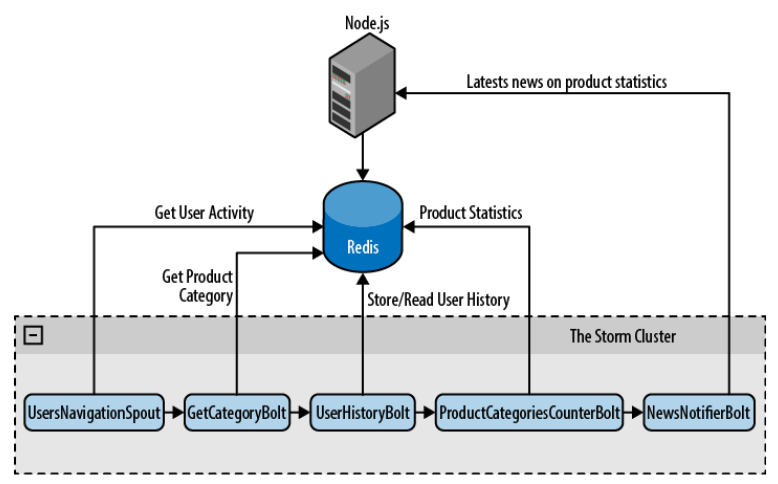
\includegraphics[width=\textwidth]{real}
\end{frame}

\begin{frame}
    \frametitle{The common things on stream data}
    \begin{itemize}
        \item A data generator, emit data point one by one.
        \item Several layers of logic to process/transform data.
        \item Each layer emit processed data point to the next layer.
    \end{itemize}
\end{frame}
\section{Structure}
\subsection{Topologies}
\begin{frame}
    \frametitle{The Structure of Storm}
    \includegraphics[width=\textwidth]{storm_struct}
\end{frame}
\begin{frame}
    \begin{itemize}
        \item Spout: Information source, emitting stream of tuples.
        \item Bolt: Logic to process or transform tuples.
    \end{itemize}
\end{frame}
\subsection{Case Study}
\begin{frame}
    \includegraphics[width=\textwidth]{stream_clus}
\end{frame}
\section{Physical Structure}
\begin{frame}
    \frametitle{physical structure}
    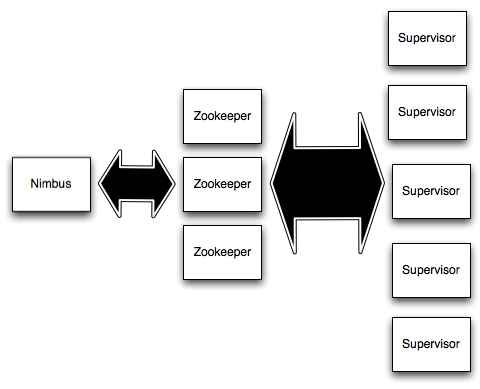
\includegraphics[width=\textwidth]{storm-cluster}
\end{frame}

\section{Implementation Details}
\subsection{Spout}
\begin{frame}
    \frametitle{Lifecycle of Spout}
    \begin{itemize}
        \item \texttt{open()} the first method called in any spout
        \item \texttt{nextTuple()}: emit values to be processed by the
            bolts.
        \item \texttt{ack(msgId)}: called after a tuple is successfully
            processed
        \item \texttt{fail(msgId)}: called when a bolt fail to process a
            tuple.
    \end{itemize}
\end{frame}

\subsection{Bolt}
\begin{frame}
    \begin{itemize}
        \item Bolts are created on the client machine, serialized into the
            topology, and submitted to the master machine of cluster
        \item The cluster launches workers that deserialized the bolt,
            call prepare on it, and then start processing tuples
        \item The most important method in bolt is \texttt{execute()}
    \end{itemize}
\end{frame}
\begin{frame}
\Huge{\centerline{Thank you}}
\end{frame}
\end{document} 
